% Exact density f(x)=2x for X=sqrt(U), 0<=x<=1.
% Shaded interval [1/4,3/4] has probability 9/16-1/16=1/2.
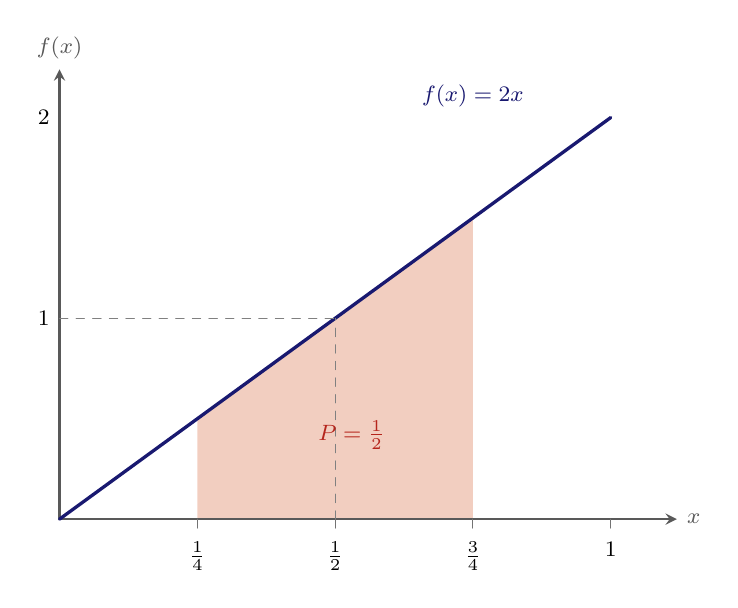
\begin{tikzpicture}[x=7.0cm,y=2.55cm,line cap=round,>=stealth]
  \fill[BrickRed!17]
    (0.25,0)--(0.25,0.5)--(0.75,1.5)--(0.75,0)--cycle;
  \draw[->,black!65,thick] (0,0)--(1.12,0) node[right,font=\footnotesize] {$x$};
  \draw[->,black!65,thick] (0,0)--(0,2.24) node[above,font=\footnotesize] {$f(x)$};
  \draw[MidnightBlue,very thick] (0,0)--(1,2);
  \draw[black!50,dashed] (0.5,0)--(0.5,1);
  \draw[black!50,dashed] (0,1)--(0.5,1);
  \foreach \x/\name in {0.25/{\frac14},0.5/{\frac12},0.75/{\frac34},1/{1}} {
    \draw[black!55] (\x,0)--(\x,-0.045);
    \node[below,font=\footnotesize] at (\x,-0.065) {$\name$};
  }
  \node[left,font=\footnotesize] at (0,1) {$1$};
  \node[left,font=\footnotesize] at (0,2) {$2$};
  \node[font=\footnotesize,anchor=west,text=MidnightBlue] at (0.64,2.11) {$f(x)=2x$};
  \node[font=\footnotesize,text=BrickRed] at (0.53,0.42) {$P=\frac12$};
\end{tikzpicture}
